\subsection{Describing bedload fluctuations: Including correlations between particle motions} 
\label{sec:ancey2008}

\citet{Ancey2006a, Ancey2008} developed a more general birth-death model in order to describe the relatively heavy tailed bedload probability distributions seen in experiments. 
In the last ten years, this model has been restated and more deeply studied by several authors \citep{Turowski2010, Heyman2013, Heyman2014a, Heyman2014, Ma2014}, and has led into exciting generalizations \citep{Turowski2010, Ancey2014, Ancey2015}. 
These are the real focus of this review. 

Instead of considering the motion of every bedload particle as an independent process involving transitions between motion and rest states, and summing a collection of these to get the total number of moving particles within the control volume, \citet{Ancey2008} consider the total number of moving particles within the control volume as a state.
In this case, instead of just two states (motion and rest), there is an infinite ladder of states ($n = 0,1,2 \dots$), each representing the number of active particles within the control volume.
The ladder of states is illustrated diagramatically in figure \ref{fig:ladder}. 

The advantage of this approach is when all particles are treated simulatenously, the transition rates can be made to depend on the number of active particles. 
The state is a collective property of the moving particles within the control volume. 
This allows interactions between particles to be introduced. 
\citet{Ancey2008} considers the population of moving particles changes due to entrainment (birth) and deposition (death), as before, but they also introduce migration processes for particles to move into (emigration) and out of (immigration) the control volume.
We note that these migration processes do not fundamentally modify the structure of the equations which result.
However, they are physically expected, so their inclusion is rational.

\begin{wrapfigure}{r}{0.5\textwidth}
  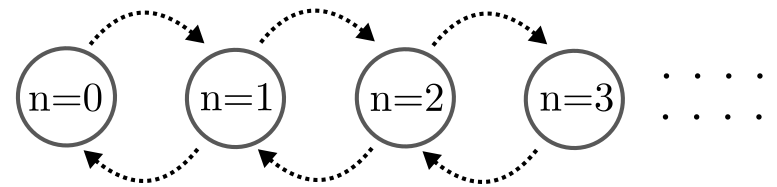
\includegraphics[width=.98\linewidth]{./figures/ancey2008.png}
  \caption{Birth, death, immigration, and emigration rates characterize the flow of probability up and down an infinite ladder of states. Each state represents $n$ particles in motion, and $n$ runs across all positive integers including zero. \label{fig:ladder} }
\end{wrapfigure} 

The key result of \citet{Ancey2008} is a successful description of wide bedload fluctuations. 
To obtain this, they made a component of the entrainment rate increase with the number of active particles. 
In effect, they introduced a positive feedback on entrainment: when more particles are in motion, entrainment becomes more likely. 
They termed this feedback term "collective entrainment".
The collective entrainment term fundamentally modifies the probability distribution of the bedload flux and lends it a wide tail, so the model is capable of describing realistically large fluctuations. 
Rather than a binomial distribution of the number of moving particles, as in \ref{eq:anceybinomial}, \citet{Ancey2008} derive a negative binomial distribution.
Within their model, collective entrainment is the source of the difference between these two distributions. 
When it is turned off, \citet{Ancey2008} reduces to \citet{Ancey2006}.  

Collective entrainment has been attributed to several physical mechanisms. 
Usually, the feedback is considered due to collisions of moving particles with the bed \citep{Ancey2008, Heyman2013, Heyman2014a} and the advection of turbulent structures implying waves of entrainment \citep{Ancey2008, Heyman2014}. 
Another consideration is that collective entrainment is the result of small avalanches, or local rearrangements of the bed surface triggered by the entrainment of an individual particle \citep{Heyman2014, Heyman2014a}. 
Entraining one grain could destabilize all of those contingent on it, so local microstructure \citep{Staron2006} may imply collective entrainment.  
These mechanisms for the collective entrainment term are reasonable, but they only hypotheses at this stage, and research is needed. 

The layout of this section is as follows: 
First, I will follow \citet{Ancey2008} to develop a master equation for the number $n$ of active particles within the control volume, obtaining a probability distribution $P(n)$. 
Then we can analyze the mean and variance of $n$ and develop the linkage to the probability distribution of the bedload flux, $P(q_s)$ using the relationship between volume and surface definitions of the flux, equation \ref{eq:fluxy}. 
This flux will be shown to link back to \citet{Einstein1950} as a limiting case. 
The magnitude of fluctuations will be considered, and we will conclude by a discussion of the model's assumptions and successes. 
In subsequent sections, we will examine generalizations of and other ways to study this model. 

\subsubsection{Master equation of the collective entrainment model} 

Consider the probability that there are $n$ particles in motion at time $t$. 
This can be denoted $P(n,t)$. 
The random variable $n$ takes on values $0,1,2,\dots$ -- non-negative integers of arbitrary magnitude. 
Each of these states has an associated probability $p_n(t)$.  
The population is subject to four transitions within a small time increment $\delta t$: 
\begin{enumerate}
\item 
Entrainment of a single bed particle (birth) can happen in time $\delta t$ with probability $\lambda_0 + \mu n$. 
The second term $\mu n$ is the collective entrainment effect. 
As the number of active particles increases, so does the rate of entrainment. 
This interaction term induces realistically wide bedload fluctuations. 
\item 
Deposition of a single bed particle can happen in $\delta t$ with probability $\sigma n$. 
This is similar to the telegrapher's process considered earlier. The rate of deposition increases with the number of active particles, just as it does implicitly in \citet{Ancey2006}. 
The deposition of each particle is independent of every other.  
\item 
Immigration of a particle from upstream into the control volume can happen in $\delta t$ with probability $\lambda_1$. 
This term does not fundamentally modify the structure of the equations we will derive for the probability distribution of the bedload rate. 
\item 
Emigration of a particle from the control volume to downstream can happen with probability $\nu$. 
This term is significant because it defines a bedload flux across a surface as in $q_s = \int dS \textbf{k} \cdot \textbf{u}_s$. 
Counting emigration events provides an alternate definition of the flux. 
This counting problem was solved by \citet{Ma2014}. 
We will consider this later. 
In this section, we will continue to interpret the flux as in section \ref{sec:fluxdef}, by converting an ensemble average to a volume average.
\end{enumerate} 
These transitions are depicted in figure \ref{fig:anceywindow}. 
The symbols of \ref{sec:ancey2008} are summarized in table \ref{tab:symbols2008}. 

\begin{wrapfigure}{l}{0.5\textwidth}
  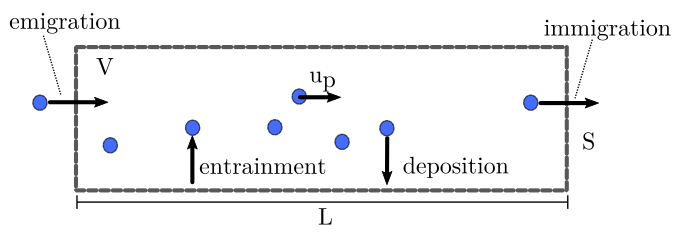
\includegraphics[width=.98\linewidth]{./figures/controlvol.png}
  \caption{As before, the model is based on analyzing the number of particles within a control volume $V$ which has downstream length $L$. Particles appear into the control volume due to entrainment and emigration. They disappear due to deposition and immigration. The downstream boundary is a stream cross section $S$.  \label{fig:anceywindow} }
\end{wrapfigure} 

We can consider the flow of probability up and down the ladder of states ($n=0,1,2,\dots$) which is induced by these transitions, entrainment (including the collective entrainment term), deposition, immigration, and emigration, using the formalism of more general Markov birth-death processes \citep{Cox1965, Pielou1977}. 
By the standard way of developing master equations \citep[e.g.][]{Cox1965}, we find an infinite system of equations for the probabilities of finding $n$ moving particles within the control volume: 
\begin{multline} P(n,t+\delta t) = \alpha \delta t (n+1)P(n+1,t) \\+  [\lambda + (n-1)\mu]\delta t P(n-1,t) \\ + [1-\delta t[\lambda + n\alpha + n\mu]]P(n,t). \end{multline}
Here $\alpha = \nu + \sigma$ summarizes the contributions of emigration and deposition, which both act to decrease the number of particles $n$, and $\lambda = \lambda_0 + \lambda_1$ summarizes the contributions of immigration and (individual) entrainment, which both act to increase the number of particles $n$. 

As $\delta t\rightarrow 0$ these equations become a hirearchy of differential-difference equations for the probabilities $P(n,t)$ of finding $n$ particles in the control volume at time $t$: 
\be \frac{d}{dt}P(n,t) = (n+1) \alpha P(n+1,t) + [\lambda + (n-1)\mu]P(n-1,t) - [\lambda +n (\alpha+\mu)]P(n,t). \label{eq:anc2008} \ee 

These master equations define a birth-death immigration emigration model \citep[e.g.][]{Cox1965, Gardiner1983}. 
It can be solved for the probabilities $P(n,t)$ by introducing the probability generating function $G(z,t) = \sum_{n=0}^\infty z^n P(n,t)$ \citep{Cox1965, Gardiner1983, Ancey2008}. 
Multiplying \ref{eq:anc2008} by $z^n$ and summing over all $n$ gives, after a careful manipulation of the sums in order to form some function of $G(z,t)$ in every term, 
\be \frac{\partial}{\partial t} G(z,t) = \lambda(z-1)G(z,t) + \{ \sigma + \mu z^2 + \nu - (\mu + \sigma + \nu)z\} \frac{\partial}{\partial z} G(z,t). \ee

In effect, the probability generating function exchanges the discrete variable $n$ for a continous variable $z$. 
This first order partial differential equation for $G$ can be solved by the method of characteristics \citep{Cox1965, Garabedian1964}. 
If there are initially $N_0$ moving particles within the control volume, the solution is 
\be G(z,t) + \Big(\frac{\alpha-\mu}{(K-1)\mu z + \alpha - K \mu}\Big)^{n+\lambda/\mu}\Big( \frac{(K\alpha-\mu)z + \alpha(1-K)}{\alpha-\mu}\Big)^n. \label{eq:generator}\ee
The factor $K$ is the autocorrelation function $K(t) = \exp(-t(\alpha-\mu)).$

A useful feature of the probability generating function is that it generates the hirearchy of probabilities $P(n,t)$ via the Taylor expansion around $z=0$: $G(z,t) = \sum_{n=0}^\infty \frac{z^n}{n!}\big(\frac{\partial}{\partial z}\big)^n G(z,t) |_{z=0}$ \citep{Cox1965}. Comparing this formula with the definition of $G$, $G(z,t) = \sum_{n=0}^\infty z^n P(n,t)$, the coefficient of $z^n$ in the power series expansion of $G(z,t)$ is  apparently $P(n,t)$. 
The generating function provides the probability of finding $n$ particles in the control volume. 

Sufficiently far from the intial time, when $K(t) \approx 0 $ in the expression of $G$, meaning $t$ is much larger than the autocorrelation time $(\alpha-\mu)^{-1}$ so the system has forgotten its initial condition, the power series expansion of $G(z,t) \rightarrow G(z)$ generates a set of stationary probabilities for the number of bedload particles in motion within the control volume: 
\be P(n) = \frac{\Gamma(r+n)}{\Gamma(r)\Gamma(1+n)} p^r (1-p)^n\text{, }n=0,1,\dots. \label{eq:negbin0}\ee
Here $r=\lambda/\mu$ and $p = 1-\mu/\alpha$ characterize the strength of the collective entrainment factor $\mu$ relative to the other transitions which act to increase ($\lambda$) or decrease ($\alpha$) the population.  
$\Gamma(x) = \int_0^\infty z ^{x-1} e^{-z} dz$ is the well-known $\Gamma$ function of mathematical physics \citep{Boas2005, Mathews1971}. It is a generalization of $x!$ to non-integer values of $x$. 
This stationary distribution only exists when $\alpha>\mu$: the rate at which sediment particles appear in the control volume is lower than their disappearance rate. 
The set of symbols introduced in the \citet{Ancey2008} formulation is summarized in table \ref{tab:symbols2008}. 

\begin{wraptable}{l}{0.5\linewidth}
\vspace{-10pt}
\caption{The parameters used in section \ref{sec:ancey2008}}\label{tab:symbols2008}
\begin{tabular}{p{3.3cm}p{3.3cm}}\\
\toprule  
Symbol & Meaning \\
\midrule
$\nu$ & emigration  \\  
$\sigma$ & deposition \\  
$\lambda_0$ & immigration  \\ 
$\mu$ & collective entrainment\\
$\lambda_1$ & entrainment\\ 
$\lambda$ &  $\lambda_0 + \lambda_1$ \\ 
$\alpha $& $\sigma+\nu$ \\
$r$ & $\lambda/\mu$ \\
$p$ & $1-\mu/\alpha$ \\
\bottomrule
\end{tabular}
\end{wraptable} 

This stationary distribution equation \ref{eq:negbin0} is the negative binomial distribution: 
\be P(n) \sim \text{NegBin}(r,p).\label{eq:negbin}\ee
It is a generalization of the binomial distribution for the number of active particles, equation \ref{eq:anceybinomial}, which was derived in the \citet{Ancey2006} paper.
The negative binomial distribution has a relatively heavy tail, so that large deviations in the number of active particles $n$ are possible. 
These large fluctuations are the result of the collective entrainment rate $\mu$, and they allow the birth-death immigration-emigration model to express bedload fluctuations of realistic magnitude. 
As we will show, they become relatively small as collective entrainment is turned off, $\mu \rightarrow 0$. 

\subsubsection{The bedload flux: wide fluctuations and the Einstein limit}

As discussed, the negative binomial distribution supports wide fluctuations, controlled by the collective entrainment parameter $\mu$. 
The mean number of particles in the control volume, taken over the distribution \ref{eq:negbin}, is 
\be \bra n \ket = \sum_{n=0}^\infty n P(n) = \frac{\lambda}{\alpha-\mu}. \label{eq:anceymean}\ee
Likewise the variance is 
\be \bra (\delta n)^2 \ket = \sum_{n=0}^\infty (n-\bra n\ket)^2 P(n) = \frac{ \lambda \alpha}{\alpha-\mu^2},\ee
which means their ratio is 
\be \frac{\bra (\delta n)^2}{\bra n\ket} = \frac{1}{1-\mu/\alpha}.\ee
It is interesting to compare this to equation \ref{eq:2006flucts} bounding the magnitude of fluctuations in the \citet{Ancey2006} model. 
In contrast, within the \citet{Ancey2008} model, the variance must exceed the mean, because as discussed, in steady state $\alpha>\mu$. 
The magnitude of fluctuations can grow arbitrarily with the collective entrainment parameter $\mu$. 
This is a coherent conclusion, since collective entrainment was introduced in order to represent the collective effects of turbulent fluctuations, collision-induced entrainment, and granular avalanches; and with the expressed intent of generating realistically wide bedload fluctuations, exceeding those of the \citet{Ancey2006} model. 

Armed with the probability distribution for the number of particles in the control volume, equation \ref{eq:negbin}, and the link between control volume and surface statistics derived in section \ref{sec:fluxdef}, equation \ref{eq:fluxy}, we can derive the probability distribution of the bedload flux in a similar way as equation \ref{eq:anceygauss}.
The number of particles in the control volume has been implicitly assumed to be infinite, so there is no need or means to take a large $N$ limit. 

Using the law for transformation of probabilities gives 
\be P(q_s) \approx \frac{\Gamma(r+\frac{Lw}{\nu_p u_s} q_s)}{\Gamma(r)\Gamma(1+\frac{Lw}{\nu_p u_s} q_s)}p^r(1-p)^{\frac{Lw}{\nu_p u_s} q_s}\ee
as the probability distribution of the bedload flux $q_s$. 

Now we link back to the \citet{Einstein1950} theory. 
Einstein considered neither immigration ($\lambda_1$), emigration ($\nu$), nor collective entrainment ($\mu$). 
When all of these parameters are set to zero, $\mu = \lambda_1 = \nu = 0$, the parameters $r$ and $p$ of the distribution \ref{eq:negbin0} become $r \rightarrow \infty$ and $p=0$. 
In this limit the distribution \ref{eq:negbin0} tends to a Poisson distribution. 

There are two ways to see this. 
The first way is to take the appropriate limits ($t \rightarrow \infty$, $\mu=lambda_1=\nu= 0$)  into the generating function \ref{eq:generator} gives 
\be G(z) = e^{-\lambda_0(z-1)/\sigma},\ee
which inverts to 
\be P(n) = \frac{(\lambda_0/\sigma)^n}{n!}e^{-\lambda_0/\sigma},\label{eq:anceypoisson}\ee
the Poisson distribution.  
The second way is to take limits of the negative binomial distribution equation \ref{eq:negbin0} directly, although this is somewhat tricky.
It involves reparameterizing the distribution by its mean value equation \ref{eq:anceymean} rather than $r$, and then taking limits, using the limit formula $e^{-x} = \lim_{s \rightarrow \infty} (1-x/s)^s$.

In either case, arriving at this Poisson distribution for $n$ in the absence of collective entrainment, we can compute the mean bedload flux using equation \ref{eq:fluxy}: 
\be \bra q_s \ket = \frac{\nu_p u_s}{L w} \sum_{n=0}^\infty n \frac{(\lambda_0/\sigma)^n}{n!}e^{-\lambda_0/\sigma} = \frac{\nu_p u_s}{L w} \frac{\lambda_0}{\sigma}. \ee
To make full contact with the Einstein-like formula of Yalin, equation \ref{eq:yalinflux}, one further step is needed. 

In the \citet{Ancey2008} collective entrainment model, there was no limitation on the number of particles within the control volume. 
In the notation of section \ref{sec:ancey2006}, this is equivalent to $N \rightarrow \infty$. 
In \citet{Ancey2006} the fraction of time spent in motion, $\xi$, referred to a single particle. 
We can show in the model under consideration that $\lambda_0/\sigma$ also represents a fraction of time spent in motion, although this is more difficult than it was in the arguments leading to the analogous conclusion for $\xi$. 

Similar to equation \ref{eq:}, one can set up a master equation to compute the distribution of time time periods that the number $n$ remains fixed while no transitions except deposition occur. 


 that particles spend in motion and to find the mean period spent in motion is $\lambda_0$. 











- this model assumes infinite sediment availability. there is no limit to n. This leads to turowski
- the flux is defined in a control volume, emigration provides a pathway to defining the flux at a point. This is Heyman 2013, and Ma 2014. 
- imagine connecting cells, this is ancey2014, which leads into Heyman 2014




\begin{comment} 




When the collective entrainment process is turned off, $\mu\rightarrow 0$, the Poisson distribution for the number of moving particles within the control volume is recovered, reproducing the limiting result of \citet{Ancey2006}, which has links to \citet{Einstein1950}. 
We will consider this limit of no collective entrainment. 
$\mu\rightarrow 0$, implies $r \rightarrow \infty$ and $p \rightarrow 1$. 
In this limit, the generating function G(z) becomes 
\be G(z) = \exp(-\frac{\lambda}{\alpha}[z-1]).\ee
Taylor expanding this generating function around $z=0$ generates the hirearchy of probabilities $\pi_n(t)$ in the limit of no collective entrainment:
\be \pi_n = \frac{(\lambda/\alpha)^n}{n!}e^{-\lambda/\alpha}.\ee
Therefore the number of particles in the control volume is Poisson distributed, in accord with the large $L$ limit of the \citet{Ancey2006} model in the previous section \ref{eq:poissonflux}. 
To complete the connection we turn off immigration ($\lambda_0=0$) and emigration ($\nu = 0$) as well, so that the distribution of the number of particles in the control volume reproduces the \citet{Ancey2006} result cleanly: 
\be \pi_n = \frac{(\lambda_1/\sigma)^n}{n!} e^{-\lambda_1/\sigma},\ee
which is the same as equation \ref{eq:poissonflux}. 
We note that immigration ($\lambda_0$ -- to move in) and emigration ($\nu$ -- to move out) do not fundamentally alter the form of the distribution.
Only collective entrainment ($\mu$) does this.  

Now we will analyze the probability distribution of bedload flux and the magnitude of its fluctuations. 
Collective entrainment develops a negative binomial distribution for the number of active particles, and in the limit of a large control volume ($L \rightarrow \infty$), the probability distribution for the number of active particles links to the probability distribution of the bedload flux via the relationship \ref{eq:fluxy} of the previous section. 
As a reminder, this relationship was derived using an artificial device. 
To develop an ensemble of particles intersecting a flow cross section $S$ with various positions $\textbf{x}$ and velocities $\textbf{u}_p$, we traded a frequentist interpretation of a conditional probability $P[\textbf{u}_p|\textbf{x}]$ for an ensemble one.
This was only valid in the limit of an infinitely long control volume $L \rightarrow \infty$. 

The \citet{Ancey2008} model reveals another way to compute the flux which does not depend on this device. 
Considering the downstream boundary of the control volume as the surface $S$ in the formula \ref{eq:anceyflux}, we can count the number of emigration events across this surface per unit time.  
There are four types of transitions in the \citet{Ancey2008} model, and these occur at random intervals. 
Counting the frequency of only one of these transitions is a non-trivial problem, and it relies on advanced techniques in stochastic mathematics. 
This counting problem was solved by \citet{Ma2014}.
They computed the bedload flux without the need for an exchange of averaging or an artificial control volume limit ($L\rightarrow \infty$). 
We will consider this work later in the review. 

For now, consider the approach of the previous section. 
The bedload flux is $q_s \approx \frac{\nu_p u_s}{L} n$, in the limit of a large control volume $L\rightarrow \infty$ and when all particles in motion approach the same velocity $u_s$.
The mean and variance of the negative binomial distribution are 
\be \bra n \ket = \frac{\lambda}{\alpha-\mu} \ee
and 
\be \bra (\delta n)^2 \ket = \frac{\lambda \alpha }{\alpha-\mu}.\ee
Because of collective entrainment, characterized by $\mu$, the variance can exceed the mean in this model: 
\be \frac{\bra (\delta n)^2 \ket}{\bra n \ket } = \frac{1}{1-\mu/\alpha}, \ee
because $1/(1-\mu/\alpha) > 1$ if $\mu > 0 $. 

By these relationships, the mean flux becomes 
\be  \bra q_s \ket = \frac{\nu_p u_s}{L} \ee,
and the magnitude of bedload fluctuations is

The Ancey et al 2008 inclusion of collective entrainment develops a Negative Binomial distribution of the bedload flux. 
Expressing the bedload flux as the number of moving particles within the control volume times their average velocity $u_p$ makes a Negative binomial distribution for bedload flux within the control volume. The mean bedload flux is $ \frac{\lambda}{\alpha-\mu} u_p $ and the variance of the flux is $ \frac{\lambda \alpha}{(\alpha-\mu)^2} u_p^2$: the fluctuations are much wider in the negative binomial distribution, meaning the inclusion of collective entrainment can model the large fluctuations observed in the \citet{Ancey2008} experiments. 

One way to view the bedload flux we just presented: it is the number of moving particles times their velocity. 
However, since this model explicitly includes downstream emigration from the control volume, there is another way to define the flux: it is the number of emigration events within a unit of time. 
Counting the number of emigration events expressed from this model within a unit time is not easy. 
\citet{Ma2014b} explored this approach to calculating the bedload flux, and I will review this in a subsequent section. 

Two key assumptions of this model are worth examining. 
These set the stage for the subsequent developments in birth-death modelling of the bedload flux which I review next. 
First, this model assumes that stationary bed particles are in infinite supply. 
This is an implicit assumption: Nothing prevents the system from entraining particles ad infinitum through the entrainment processes characterized by rates $\lambda_0$ and $\mu$. 
Second, the model considers sediment transport in an isolated control volume, so the sediment flux is described probabilistically in a locality, but spatial correlations cannot be accounted for: the flux upstream of the control volume is also a fluctuating quantity, implying spatial correlations through immigration events into the control volume considered in this model.

These two observations support two of the more recent developments to the \citet{Ancey2008} birth-death immigration-emigration model: \citet{Turowski2009} generalized this model to finite bed material in order to describe transport within semi-alluvial bedrock environments, where alluvial deposits of limited quantity sit on top of bedrock. When all available particles are entrained and moved away from the control volume, there are none left to entrain, so the entrainment process is turned off. 
Likewise, \citet{Ancey2010, Ancey2014,Ancey2015} extended the birth-death process within a control volume as I reviewed here to an array of spatially distributed control volumes (cells). 
They showed that immigration and emigration processes between cells set up a bedload diffusion, and they connected this theory with earlier sediment diffusion theories by deriving an Exner type equation of sediment diffusion. 
I will now review each of these developments in turn. 
\end{comment} 

